
%%%%%%%%%%%%%%%%%
% Version: Final - Mar 26
%%%%%%%%%%%%%%%%%

\documentclass[runningheads,a4paper]{llncs}

% Packages
\usepackage{amsmath}
\usepackage{amssymb}
\setcounter{tocdepth}{3}
\usepackage{graphicx}
\usepackage{epstopdf}
\usepackage{url}

\usepackage{array}
\usepackage{multirow}
\usepackage{rotating}
\usepackage{verbatim} 

\urldef{\mailsa}\path|{egg,igcf}@cin.ufpe.br|    
\urldef{\mailsb}\path|christoph.dieterich@mdc-berlin.de|  
\newcommand{\keywords}[1]{\par\addvspace\baselineskip
\noindent\keywordname\enspace\ignorespaces#1}

\begin{document}

\mainmatter

% Title
\title{Prediction of Transcription Factor Binding Sites by Integrating DNase digestion and Histone Modification}

% A short form should be given in case it is too long for the running head
\titlerunning{Prediction of TFBS by Integrating DNase and Histone Modification}

% Authors
\author{Eduardo G. Gusm\~{a}o$^a$\and Christoph Dieterich$^b$ \and Ivan G. Costa$^a$}

% Affiliations
\institute{$^a$Center of Informatics, Federal University of Pernambuco, Recife, Brazil\\
  $^b$ Berlin Institute for Medical Systems Biology, Berlin, Germany\\
  \mailsa,\mailsb\\
%\url{http://www.cin.ufpe.br/~igcf}
}

\maketitle

\begin{abstract}

  The identification of cis-acting elements on DNA is crucial for the
  understanding of the complex regulatory networks that govern many
  cell mechanisms. However, this task is very complex since it is
  estimated that there are 1500 different transcription factors (TFs) 
  in the human genome, each of which can bind to multiple loci directly or indirectly. The
  standard computational approach is the use of a position weight
  matrix (PWM) to represent the binding preference of a transcription
  factor and the use of statistical procedures to detect genomic
  regions with high binding scores. Given the small and degenerate
  signals of most PWMs, such approach suffers from a very high number
  of false positive hits. Current research has proven that genome wide
  assays reflecting open chromatin, such as DNase digestion or histone
  modifications, can improve sequence based detection of the binding
  location of transcription factors that are active in a particular
  cell type.  We propose here a Multivariate Hidden Markov Model that
  is able to improve the prediction of transcription factor binding
  locations by integrating DNase digestion and histone modification
  data. Our methodology improves sensitivity, in comparison to
  existing methods, with little or no effect at specificity rates.
  This study shows that it is possible to improve predictability power
  of cis-acting elements by correctly integrating DNase and histone
  modification data, allowing for more sophisticated studies using a
  larger set of epigenetic signals.  \keywords{cis-regulatory
    elements, DNase I-hypersensitive sites, histone modifications,
    hidden markov models}
\end{abstract}

\section{Introduction}

Complex regulatory networks govern many critical cell mechanisms such
as proliferation, development, differentiation, aging and apoptosis.
The regulatory mechanism consists of a large number of different
components that may play a role in numerous regulatory pathways
\cite{encode2012}. Examples of these components are trans-acting
elements (or transcription factors), cis-acting elements (such as
enhancers, silencers and insulators) and epigenetic factors (such as
histone modifications, chromatin remodeling complexes and DNA
methylation), each collaborating in the orchestration of proper
temporal and spatial expression required by ubiquitous, common or
cell-specific processes \cite{maston2006}. Consequently, it is crucial
to identify these regulatory elements in order to understand their
role in each cell's regulatory network and comprehend diseases caused
by deregulation.

The identification of cis-acting elements, which transcription factors
bind to, can be a particularly daunting task since it is estimated
that there are 1500 factors in the human genome \cite{boyle2011}.
Furthermore, transcription factor binding sites (TFBSs) are generally
small, in the range of 6--12 bp with binding specificity dictated by
no more than 4--6 positions within this site~\cite{maston2006}, and
only a subset of them are active during a current cell state
\cite{cuellar2012}. In addition, many transcription factors may have
multiple binding sites with different motifs \cite{maston2006}; and
some of these elements may bind to the DNA by indirectly binding with
another factor or protein complex.  The standard computational
approach --- motif matching --- uses position weight matrix (PWM)
representation of transcription factor binding preference followed by
a statistical procedure to detect genomic regions with a high binding
score for a particular TF~\cite{stormo2000}. Nevertheless, motif matching is highly
dependent on the strength of the matching algorithm, it can not
distinguish between active and non-active binding sites and presents a
high number of false positives as motifs are mostly small and
degenerate~\cite{maston2006}.  An alternative are Chromatin
immunoprecipitation assays, which can be applied to finding binding
sites on a genome-wide fashion (ChIP-Seq).  However such experiments
are condition-specific, fails for some particular TFs and are 
experimentally and financially demanding~\cite{park2009}.

Current research has proven that genome wide assays reflecting open
chromatin states, such as DNase digestion data
(DNase-Seq)~\cite{boyle2011,cuellar2012} or histone modifications
(ChIP-Seq)~\cite{hon2009}, can improve sequence based detection of the
binding location of transcription factors that are active in a
particular cell type. The rational of such approaches is to restrict
the sequence based search of binding sites to genomic regions where
either DNase digestion or histone marks indicates the chromatin is
open and accessible for TF binding. Traditional open chromatin assays
with DNase I as cleavage agent have long been used to characterize
hypersensitive sites, i.e. genomic regions with many sites digested by
DNase, and it is considered a high-accuracy and high-resolution
technique \cite{gross1988}. This technique can be combined with
high-throughput sequencing to provide genome-wide maps of open
chromatin of a particular cell type~\cite{crawford2004}.  Similarly,
ChIP-Seq assays can be used to measure patterns of histone variants
and their post-translational modifications (such as acetylation and
methylation) in different cell lines. Many studies have shown clear
chromatin signatures for particular regulatory regions, such as active
promoters and enhancers, and have suggested the application of their
findings to predict elements of the regulatory
mechanism~\cite{cuellar2012,hon2009,barski2007}.

We propose here a multivariate Hidden Markov Model (HMM) that is able
to identify transcription factor binding sites (TFBSs) by integrating
DNase digestion data and histone modification data of a particular
cell type. The method outperforms previous models based on HMMs, which
made predictions either with histone modification~\cite{hon2009} or
DNase digestion~\cite{boyle2011} alone.  Moreover, we also propose
here a procedure to estimate the HMM parameters without necessity of traditional
DNase digestion data as in~\cite{boyle2011}. We evaluate the
method by using DNase digestion data and histone modifications from
the leukemia cell line K562 to predict TFBSs of four TFs: ATF3, CTCF,
GABP and REST.

\subsection{Related Work}

Boyle et al \cite{boyle2011} proposed an HMM model, which used DNase-seq data
to predict TFBSs that are active in a particular cell type. The HMM parameters were obtained
with a manual annotation of DNase hypersensitivity sites. Won et al
\cite{won2010} used a multivariate HMM model with scores produced by
motif matching with PWMs and ChIP-seq signals of histone modifications
to predict binding sites of individual transcription factors. Cuellar-Partida et al \cite{cuellar2012} 
described a method for combining epigenetic data with standard DNA sequence on a Bayesian approach. 
Pique-regi et al \cite{pique2011} created an
algorithm that combines genomic sequence information (such as
conservation) with cell-specific experimental data (such as DNase and
histone modifications) using a Bayesian approach.

\section{Materials and Methods}

The proposed methodology works as follows. As a first step, we perform
a simple motif matching experiment to detect sequence based
predictions of TFBSs (Section~\ref{sc:tfbs}). From this point, we 
will use the nomenclature Motif Predicted Binding Sites (MPBSs) to define 
these sequence based TFBSs candidates. Next, we
detect DNase hypersensitive regions of the target cell type
(Section~\ref{sc:dhr}). Our search for TFBSs will be restricted to this region only.  
Then, high-resolution signal of the DNase digestion and
histone modification data from the target cell type are used as input
for the HMM (Section~\ref{sc:hrs}), which was previously trained using
manually annotated footprint regions or regions around sequence based
TFBS predictions (Section~\ref{sc:hmm}). The HMM uses DNase digestion
and histone modification signals to detect footprint regions, 
i.e. small regions within DNase hypersensitive sites
where TFs are likely to bind. We regard as `predictions', MPBSs
that matche footprint regions. Finally, we use ChIP-seq data for 
specific TFBSs to validate the accuracy of the HMMs (Section~\ref{sc:gs}).

\subsection{Motif Matching\label{sc:tfbs}}

All the PWMs were obtained from one of these repositories:
Jaspar~\cite{byrne2008}, Transfac~\cite{matys2006} and
Uniprobe~\cite{newburger2009}
, and a high-quality CTCF motif was
obtained from Renlab \cite{kim2007}. A PWM is a representation for
sites of preferred binding by specific transcription factors that
consists of evaluated levels of affinity for each position of the
motif and for each nucleotide. There are some redundancies among
these databases, i.e. there are many motifs for the same factor, but
as each one has its own quality that depends on the particular study
that generated it, we analyzed each one separately. All the motifs
were matched against the complete genome using the motif matching tool
available in Biopython \cite{cock2009} to produce a bit score. Next,
matches (MPBSs) were discarded if they had scores lower than the maximum
between 70\% of the highest possible bit score and 90\% of the
difference between the highest possible or the lowest possible bit
score \cite{boyle2011}. We would like to state that we are aware that
more robust motif matching algorithms exist and our intention on using
these criteria is to replicate \cite{boyle2011} providing a reliable 
comparative scenario.

\subsection{Detection of DNase Hypersensitive Regions\label{sc:dhr}}

DNase Hypersensitive Regions were detected as described in the ENCODE
project~\cite{encode2012}. Briefly, the regions of significant
enrichment of DNase digestion tags (HS regions) were identified using
the F-seq method \cite{boyle2008b}. This computational tool identifies
regions of high density of sequence reads by applying a Parzen window
methodology and considering a random background distribution of reads.
Then, the resulting distribution of F-seq scores (at bp resolution)
was fitted to a gamma distribution and a P-value of 0.05 was used to
discretely define the regions more likely to be in open chromatin
state. For the cell line K562, there are 133.372 DNase
hypersensitivity regions.

\subsection{DNase and Histone Modification High-Resolution Signal Generation\label{sc:hrs}}

We use high-resolution signals of DNase digestion and histone
modification as input for our HMMs. For DNase data, we apply the same
procedure as proposed in~\cite{boyle2011}.  First, we counted all the
5$^\prime$ bp (corresponding to the exact position at which DNase I enzyme
has nicked the DNA) generating a digestion signal at the bp
resolution. Then, this signal was normalized by dividing each bp count
by the mean of all non-zero entries in a 1kb window surrounding that
bp. Finally, the slope of this normalized signal was obtained by the
Savitzky-Golay method. In this method, the data are fitted to a second
order polynomial and a convolution method is applied to access the
first derivative based on a window size of 8bp.

This signal corresponding to the slope of the normalized curve assumes
positive values when there is an increase and negative values when
there is a decrease. The higher the slope signals are, the steeper the normalized
increase is, and the lower the slope signals are, the steeper the decrease is. 
This strategy is performed to access the
DNase footprint patterns previously described, where the transcription
factor binding sites are clearly characterized as a depletion in the
DNase I digestion between two peaks \cite{boyle2011}. Consequently,
the slope signal of the read counts permits the
training of an HMM that has the necessary states to capture this
peak-dip-peak pattern. See Figure~1 rigth for an example of DNase
signals.

The histone modification signal was based at the read-counts level. We
extended each histone fragment mapped to the genome, which originally
contained 36bp, to exactly 200bp. The resulting signal consisted of
the natural logarithm of the counted reads. The log step is done to
soften the parameter values of the HMM between different states and
make its distribution closer to normal. For this experiments, we have
used histone modifications with a known role for indicating active
regulatory regions: H3k4me2, H3k4me3, H3k9ac and the histone variant
H2A.Z.

\subsection{Detection of Footprints with HMMs\label{sc:hmm}}

A five-state bivariate emission HMM was used to integrate the signal
of DNase and one histone modification to predict open chromatin (see
Figure~1 left for the HMM topology). The first state (labeled BACK)
represents the background of the HS site. Typically, this state
recognizes regions of low or moderate DNase digestion and low histone
signal. The second state (HH) was created to capture the high histone
marks that occur at the surroundings of the DNase HS core (region
where there are higher concentrations of peaks). The rest of the model
followed the methodology described in \cite{boyle2011}. The UP state
recognizes increasing DNase digestion peaks while DOWN state
recognizes decreasing signals. The footprint state (FP) is
characterized then after the DOWN state and before another UP state,
according to the peak-dip-peak trend. The most noticeable difference
between our bivariate model and Boyle et al's univariate model is that, in our model, the HMM enters in
the open chromatin identification states (UP, DOWN and FP) only after
a significant increase in the histone modification signal. Moreover,
we expect small levels of histone marks at the FP state (see average
signals of the DNA digestion and of the H2A.Z histone mark for a 1000bp 
region centered at the 100 top scored MPBSs at Figure~1 right). The posterior 
probability was used to determine the most probable state.

We performed two different training approaches. The first one, used by
Boyle et al \cite{boyle2011}, consists of training via
maximum-likelihood algorithm an HMM model with a manually annotated
DNase hypersensitive region corresponding to the promoter region of
the fragile X mental retardation 1 (FMR1) gene \cite{drouin1997}. This
model is then used to annotate the 1000 top scored HS regions of the
chromossome 6, with the assumption that these strong sites would
consist of ubiquitous regulatory features. A final HMM model is
obtained after re-estimation of parameters with these annotated sites.
We will refer to this aproach as FMR1 in the subsequent text. We also
developed a novel approach that requires no high resolution initial
footprint region. We matched all the motifs in jaspar, transfac and
uniprobe repositories against the 10 top scored HS regions using the
STAMP algorithm~\cite{mahony2007}.  These sites were then annotated,
used to train the HMM model and excluded from further analysis.  The
General Hidden Markov Model (GHMM) python binding package was used to
implement the HMMs~\cite{ghmm2012}.

\begin{figure}
\vspace{0.0cm}
    \centering
    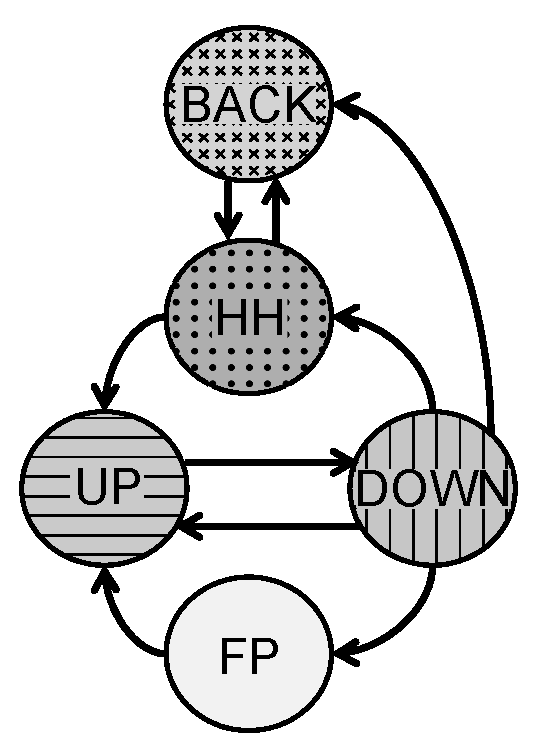
\includegraphics[width=0.25\textwidth]{Figs/Fig1a}
    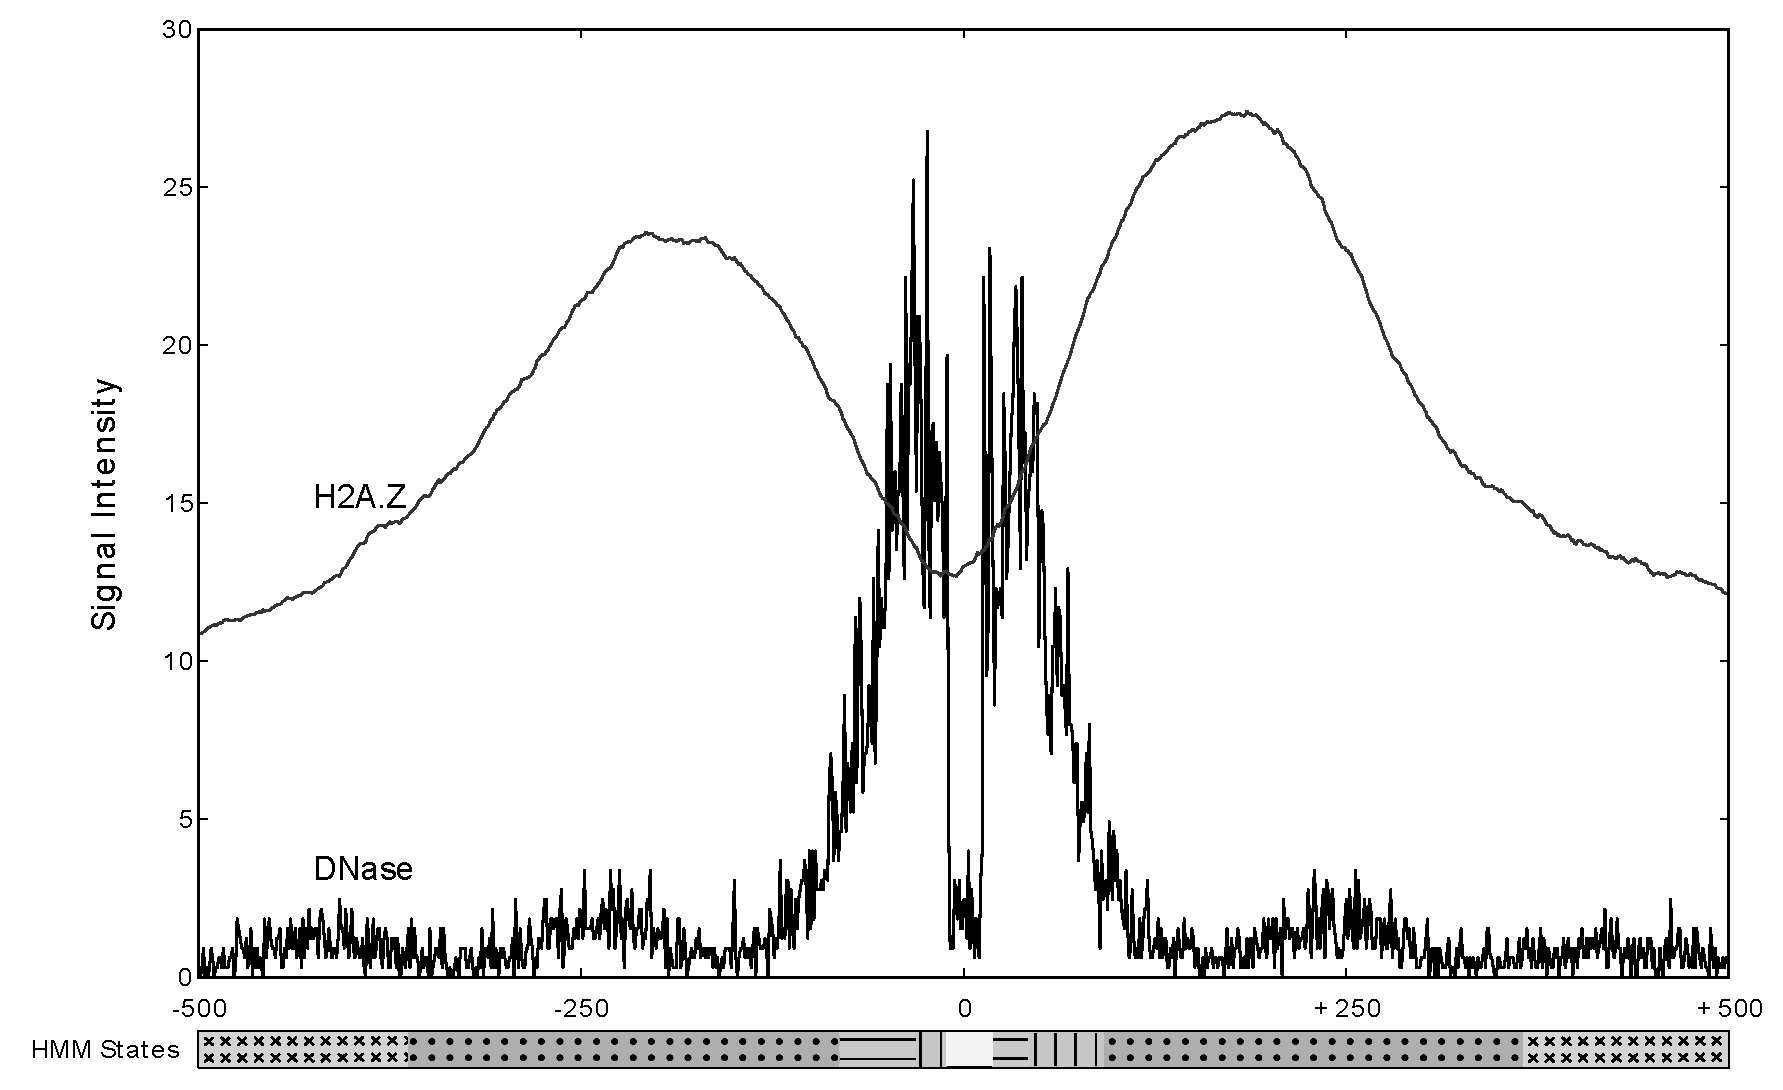
\includegraphics[width=0.74\textwidth]{Figs/Fig1b}

    \caption{HMM topology (left) and the mean DNase digestion and H2A.Z
      histone signal for a 1000bp region centered at the 100 top scored 
      MPBSs within a ChIP-seq enriched region for CTCF (right). We
      display below an example plot of the most probable HMM states for the mean
      signals.}
    \label{Label1}
\vspace{0.0cm}
\end{figure}

\subsection{TFBS Gold Standard\label{sc:gs}}

The gold standards were defined as in previous studies
\cite{boyle2011,cuellar2012}. We use the TFBS predictions from
genome-wide ChIP-Seq of the leukemia cell line K562 provided by ENCODE
(data tracks HAIB, SYDH and UTA) for the factors ATF3, CTCF, GABP and REST 
(see ENCODE project for exact details on TFBS prediction).

After performing the motif matching, the MPBSs that contained
ChIP-seq evidence were considered positives and those which did not
contain such evidence were considered negatives. Therefore, we can
state the following: MPBSs that contained ChIP-seq evidence and were
predicted by the model are considered true positives, MPBSs that
contained ChIP-seq evidence but were not predicted by the model are
false negatives, MPBSs that did not contain ChIP-seq evidence but
were identified by the model are false positives and MPBSs that did
not contain either ChIP-seq evidence or footprint evidence are
considered true negatives.  This criterion allows a quantitative
measurement of the performance of footprinting algorithms. 
We calculated the sensitivity (Sn) as $ TP/(TP+FN) $,
specificity (Sp) as $ TN/(TN+FP) $, positive predictive value (Pp) as
$ TP/(TP+FP) $, negative predictive value (Np) as $ TN/(TN+FN) $ and
correct rate (Cr) as $ (TP+TN)/(TP+FN+TN+FP) $.

% 3. Results
\section{Results and Discussion}

% Present the factors and histone modifications
We focused our analysis on four different transcription factors: ATF3
(cyclic AMP-dependent transcription factor), CTCF (CCCTC-binding
factor), GABP (GA-binding protein) and REST (or NRSF). We use one ATF3
motif (transfac), two CTCF motifs (jaspar and renlab), one GABP motif
(jaspar) and two REST motifs (jaspar and transfac), making a total of
6 motifs. We performed the analyis by combining the DNase digestion
with either the histone variant (H2A.Z) or one of the four histone
modifications (H3K4me2, H3K4me3 abd H3K9ac). For simplicity, we will
refer to both histone variants and histone modifications as histone
modifications.

To integrate histone modification into our model, we analyzed their
patterns surrounding known TFBSs (Figure 1 (right)). This figure show
a clear peak-dip-peak trend for both the H2A.Z and DNase digestion.
However, unlike DNase digestion signal, histone modification signal
presents a smooth appearance and its dips usually span over 
longer regions since ChIP-seq methodology provides
lower resolution than DNase-seq. Moreover the decrease in histone
levels are simultaneous to the increase of the DNase digestion sites.
Similar profiles were obtained for other TFs and histone modifications.
 
After the analysis of the histone signal, eight HMM models were created
(with the topology depicted in Fig. 1 left). These models
correspond to the FMR1-based training and STAMP-based training of four
models, each one composed by DNase-seq data plus one of the histone
modifications. As an initial study, we did not create models with
dimension larger than 2 as that would increase significantly the
chance of overfitting. Also, we wanted to compare the predictive power of
each histone modification separately. We then performed the
footprinting in the statistically determined HS regions of cell line
K562.

The Table 1 exhibits results for the accuracy assessment criteria described in Section~\ref{sc:gs}. 
The statistics are evaluated in order to measure the capability of both DNase only and DNase combined with histone modifications, to predict CTCF motif from jaspar repository. 

\renewcommand{\multirowsetup}{\centering}
\begin{table}
\vspace{0.0cm}
\begin{center}
\caption{Results on CTCF (jaspar) for all models trained with either FMR1 or STAMP methodologies. For each statistic, the best result is marked in bold}
\renewcommand{\arraystretch}{1.2}
  \begin{tabular}{>{\centering\arraybackslash} m{2.0cm}
                  >{\centering\arraybackslash} m{1.5cm}
                  >{\centering\arraybackslash} m{1.5cm}
                  >{\centering\arraybackslash} m{1.5cm}
                  >{\centering\arraybackslash} m{1.5cm}
                  >{\centering\arraybackslash} m{1.5cm}
                  >{\centering\arraybackslash} m{1.5cm} }
  % Header
  \hline
  Model & Train & Sn & Sp & Pp & Np & Cr \\
  % Boyle
  \hline
      \multirow{2}{*}{DNase only} 
      & FMR1  & 29.45 & 99.59 & {\bf 99.87} & 11.35 & 35.28 \\
      & STAMP & 26.08 & {\bf 99.86} & 99.95 & 10.91 & 32.21 \\
  % H2A.Z
  \hline
      \multirow{2}{*}{H2A.Z} 
      & FMR1  & 50.33 & 97.93 & 99.63 & 15.16 & 54.29 \\
      & STAMP & 71.80 & 94.74 & 99.34 & 23.35 & 73.71 \\
  % H3K4me2
  \hline
      \multirow{2}{*}{H3K4me2} 
      & FMR1  & 63.71 & 95.85 & 99.41 & 19.32 & 66.38 \\
      & STAMP & 74.76 & 94.74 & 99.37 & 25.39 & 76.42 \\
  % H3K4me3
  \hline
      \multirow{2}{*}{H3K4me3} 
      & FMR1  & 65.13 & 96.13 & 99.46 & 19.99 & 67.71 \\
      & STAMP & {\bf 75.45} & 94.33 & 99.32 & {\bf 25.83} & {\bf 77.02} \\
  % H3K9ac
  \hline
      \multirow{2}{*}{H3K9ac} 
      & FMR1  & 60.95 & 96.68 & 99.51 & 18.33 & 63.92 \\
      & STAMP & 74.96 & 94.33 & 99.32 & 25.46 & 76.57 \\
  \hline
  \end{tabular}
\end{center}
\vspace{0.0cm}
\end{table} 

The inclusion of any histone modifications
always outperforms the DNase only HMM. The latter, usually achieves high
specificity but low sensitivity. The inclusion of histone
modifications improves drastically the sensitivity with a small
decrease in specificity. Moreover, the STAMP training performed better
than FMR1 training when histone signal were included. All models
achieved around 75\% of correct predictions, increasing about 40\% in
sensitivity while losing, at most, 5\% in specificity.



Table 2 allows for a wider range of comparisons. For renlab's CTCF
motif and for both REST motifs, the inclusion of histone modification
data have shown considerably better results than DNase only.

\begin{table}
\vspace{0.0cm}
\begin{center}
  \caption{Results on ATF3, CTCF, GABP and REST factors, for DNase
    only model trained with FMR1 and our model trained
    with STAMP. For each statistic, the best result(s) is(are) marked
    in bold}
\renewcommand{\arraystretch}{1.2}
  \begin{tabular}{>{\centering\arraybackslash} m{0.3cm}
                  >{\centering\arraybackslash} m{0.5cm}
                  >{\centering\arraybackslash} m{1.0cm}
                  >{\centering\arraybackslash} m{1.8cm}
                  >{\centering\arraybackslash} m{1.8cm}
                  >{\centering\arraybackslash} m{1.8cm}
                  >{\centering\arraybackslash} m{1.8cm}
                  >{\centering\arraybackslash} m{1.8cm} }
                  %>{\centering\arraybackslash} m{1.8cm} }
  % Header Row 1
  \hline
      \multirow{1}{*}{} &
      \multirow{1}{*}{} &
      \multirow{1}{*}{} & 
      \multirow{2}{*}{DNase only} & 
      \multicolumn{4}{c}{\centering New Model }\\
  % Header Row 2
  \cline{5-8}
      & & & &
      \multicolumn{1}{c}{H2A.Z}    & 
      \multicolumn{1}{c}{H3K4me2}  & 
      \multicolumn{1}{c}{H3K4me3}  & 
      \multicolumn{1}{c}{H3K9ac}   \\ 
      %\multicolumn{1}{c}{H4K20me1} \\
  % ATF3_t1
  \hline
      \multirow{5}{*}{\begin{sideways}ATF3\end{sideways}} &
      \multirow{5}{*}{\begin{sideways}(Transfac)\end{sideways}}
      &   Sn & 58.75 & 70.00 & 76.25 & {\bf 77.50} & 67.50 \\ %81.25 \\
      & & Sp & {\bf 96.80} & 90.32 & 89.68 & 89.32 & 89.88 \\ %95.45 \\
      & & Pp & {\bf 10.28} &  4.31 &  4.41 &  4.33 &  3.99 \\ %10.03 \\
      & & Np & 99.73 & 99.79 & {\bf 99.84} & {\bf 99.84} & 99.77 \\ %99.88 \\
      & & Cr & {\bf 96.57} & 90.19 & 89.60 & 89.25 & 89.74 \\ %95.37 \\
  % CTCF_r1
  \hline
      \multirow{5}{*}{\begin{sideways}CTCF\end{sideways}} &
      \multirow{5}{*}{\begin{sideways}(Ren)\end{sideways}} 
      &   Sn & 29.68 & 69.16 & 72.51 & {\bf 72.98} & 72.27 \\ %25.74 \\
      & & Sp & {\bf 98.40} & 88.26 & 87.82 & 87.45 & 88.11 \\ %96.57 \\
      & & Pp & {\bf 98.82} & 96.38 & 96.42 & 96.34 & 96.49 \\ %97.14 \\
      & & Np & 23.64 & 38.77 & 41.42 & {\bf 41.73} & 41.29 \\ %22.35 \\
      & & Cr & 42.13 & 72.62 & 75.29 & {\bf 75.60} & 75.14 \\ %38.58 \\
  % GABP_j1
  \hline
      \multirow{5}{*}{\begin{sideways}GABP\end{sideways}} &
      \multirow{5}{*}{\begin{sideways}(Jaspar)\end{sideways}} 
      &   Sn & 27.90 & 46.32 & 50.87 & {\bf 53.11} & 42.19 \\ %41.97 \\
      & & Sp & {\bf 99.77} & 94.96 & 94.55 & 94.37 & 94.49 \\ %99.02 \\
      & & Pp & {\bf 91.84} & 46.27 & 46.61 & 46.91 & 41.74 \\ %79.97 \\
      & & Np & 93.66 & 94.97 & 95.36 & {\bf 95.56} & 94.58 \\ %94.80 \\
      & & Cr & {\bf 93.62} & 90.80 & 90.81 & 90.84 & 90.01 \\ %94.13 \\
  % REST_j1
  \hline
      \multirow{5}{*}{\begin{sideways}REST\end{sideways}} &
      \multirow{5}{*}{\begin{sideways}(Jaspar)\end{sideways}} 
      &   Sn & 20.49 & {\bf 55.21} & 55.04 & 55.04 & {\bf 55.21} \\ % 9.91 \\
      & & Sp & {\bf 96.67} & 95.00 & 95.00 & 95.00 & 95.00 \\ %98.33 \\
      & & Pp & 99.18 & {\bf 99.54} & {\bf 99.54} & {\bf 99.54} & {\bf 99.54} \\ %99.15 \\
      & & Np &  5.82 &  {\bf 9.73} &  9.69 &  9.69 &  {\bf 9.73} \\ % 5.25 \\
      & & Cr & 24.17 & {\bf 57.13} & 56.97 & 56.97 & {\bf 57.13} \\ %14.18 \\
  % REST_t1
  \hline
      \multirow{5}{*}{\begin{sideways}REST\end{sideways}} &
      \multirow{5}{*}{\begin{sideways}(Transfac)\end{sideways}} 
      &   Sn & 31.78 & {\bf 69.44} & 68.95 & 69.19 & {\bf 69.44} \\ %13.94 \\
      & & Sp & {\bf 100.0} & {\bf 100.0} & {\bf 100.0} & {\bf 100.0} & {\bf 100.0} \\ %100.0 \\
      & & Pp & {\bf 100.0} & {\bf 100.0} & {\bf 100.0} & {\bf 100.0} & {\bf 100.0} \\ %100.0 \\
      & & Np &  3.13 &  {\bf 6.72} &  6.62 &  6.67 &  {\bf 6.72} \\ % 2.49 \\
      & & Cr & 33.25 & {\bf 70.10} & 69.62 & 69.86 & {\bf 70.10} \\ %15.79 \\
  \hline
  \end{tabular}
\end{center}  
\vspace{-0.3cm}
\end{table}  

We must
notice that, although our models have increased the sensitivity for
ATF3 and GABP, the correct rate was lower than DNase only model. This
happened due to the great quantity of negative instances, i.e. 
MPBSs without ChIP-seq evidence. However, the
use of histone modification data presented better results at average,
while the accuracy of DNase only model was highly dependent of the
factor. Another relevant aspect is the fact that histones modifications
have overall close results with H3K4me3, H3k9ac and H2A.Z as best
results for distinct factors. These histone modifications, which are
well known to be related to active promoter regions, can be
alternatively used for the task of predicting active TFBSs.

% Final Remarks
\section{Final Remarks}

% Conclusion - talking about what was done
In this work, we proposed a novel multivariate emission HMM method to
predict TFBSs based on DNase I digestion patterns and histone
modification data. We analyzed the patterns of histone modifications
on various factors and determined the modification types that best
suit our interests in this exploratory study. We compared our model
with a previously suggested model that uses only DNase digestion as
input and demonstrated that, in most cases, ours is as good as or
better. This study showed that it is possible to combine different
epigenetic signals to improve the precise identification of TFBSs
without losing much specificity.

% Future work
In future studies, the number of cell lines, histone modifications and
tested factors will be increased. An initial plan would consist of extending
the bivariate model to more than two dimensions. However, this has to
be done using more careful strategies since the chance of overfitting
is significantly higher. In addition, the model can be created with
other types of epigenetic data or even genomic data, that are not
cell-type specific (such as sequence conservation or PWM motif
matching score). We also plan to analyze the accuracies of our model
considering epigenetic relationships between histone modifications and
cis-acting regulatory element type (enhancer, silencer, insulator and
others). Furthermore, we intent to keep researching training methodologies
that do not require laborious manual annotations and are capable of
describing general and specific patterns in data. Finally, we plan to
investigate more thoroughly which epigenetic signals are better predictors of TFBSs
given a particular cell line and factor and draw conclusions about the generalization
capability of these epigenetic features.

\subsubsection*{Acknowledgments.} We would like to thank Marc\'{i}lio
C.P. de Souto and Tha\'{i}s G. do R\^{e}go for sharing some valuable
information and for making helpful suggestions.

\subsubsection*{Funding.}  This work has been partially supported by Brazilian research agencies: FACEPE, CNPq and CAPES.

\begin{thebibliography}{4}

%[ENCODE 2012]
\bibitem{encode2012} Rosenbloom, K.R., Dreszer, T.R., Long, J.C., Malladi, V.S., Sloan, C.A., Raney, B.J., Cline, M.S., Karolchik, D., Barber, G.P., Clawson, H., Diekhans, M., Fujita, P.A., Goldman, M., Gravell, R.C., Harte, R.A., Hinrichs, A.S., Kirkup, V.M., Kuhn, R.M., Learned, K., Maddren, M., Meyer, L.R., Pohl, A., Rhead, B., Wong, M.C., Zweig, A.S., Haussler, D., Kent, W.J.: ENCODE Whole-Genome Data in the UCSC Genome Browser: Update 2012. Nucleic Acids Res. 40(Database issue), D912--D917 (2012)

%[Maston GA et al 2006]
\bibitem{maston2006} Maston, G.A., Evans, S.K., Green, M.R.: Transcriptional Regulatory Elements in the Human Genome. Annu Rev Genomics Hum Genet. 7, 29--59 (2006)

% [Boyle AP et al 2011]
\bibitem{boyle2011} Boyle, A.P., Song, L., Lee, B.K., London, D., Keefe, D., Birney, E., Iyer, V.R., Crawford, G.E., Furey, T.S.: High-Resolution Genome-Wide In Vivo Footprinting of Diverse Transcription Factors in Human Cells. 
Genome Res. Biol. 21(3), 456--464 (2011)

%[Cuellar-Partida G et al 2012]
\bibitem{cuellar2012} Cuellar-Partida, G., Buske, F.A., McLeay, R.C., Whitington, T., Noble, W.S., Bailey, T.L.: Epigenetic Priors for Identifying Active Transcription Factor Binding Sites. Bioinformatics. 28(1), 56--62 (2012)

%[Stormo GD 2000]
\bibitem{stormo2000} Stormo, G.D.: DNA Binding Sites: Representation and Discovery. Bioinformatics. 16(1), 16--23 (2000)

%[Park PJ 2009]
\bibitem{park2009} Park, P.J.: ChIP-seq: Advantages and Challenges of a Maturing Technology. Nature Reviews Genetics. 10(10), 669--680 (2009)

%[Hon G et al 2009]
\bibitem{hon2009} Hon, G., Wang, W., Ren, B.: Discovery and Annotation of Functional Chromatin Signatures in the Human Genome. PLoS Computational Biology. 5(11), e1000566 (2009)

%[Gross DS and Garrard WT 1988]
\bibitem{gross1988} Gross, D.S., Garrard, W.T.: Nuclease Hypersensitive Sites in Chromatin. Ann. Rev. Biochem. 57, 159--197 (1988)

% [Crawford GE et al 2004]
\bibitem{crawford2004} Crawford, G.E., Holt, I.E., Mullikin, J.C., Tai, D., National Institutes of Health Intramural Sequencing Center, Green, E.D., Wolfsberg, T.G., Collins, F.S.: Identifying Gene Regulatory Elements by
Genome-Wide Recovery of DNase Hypersensitive Sites. PNAS. 101(4), 992--997 (2004)

%[Barski A et al 2007]
\bibitem{barski2007} Barski, A., Cuddapah, S., Cui, K., Roh, T., Schones, D.E., Wang, Z., Wei, G., Chepelev, I., Zhao, K.: High-Resolution Profiling of Histone Methylations in the Human Genome. Cell. 129(4), 823--837 (2007)

%[Won K et al 2010]
\bibitem{won2010} Won, K., Ren, B., Wang, W.: Genome-Wide Prediction of Transcription Factor Binding Sites Using an Integrated Model. Genome Biology. 11(1), R7 (2010)

%[Pique-Regi R et al 2011]
\bibitem{pique2011} Pique-Regi, R., Degner, J.F., Pai, A.A., Gaffney, D.J., Gilad, Y., Pritchard, J.K.: Accurate Inference of Transcription Factor Binding from DNA Sequence and Chromatin Accessibility Data. Genome Res. 21(3), 447--455 (2011)

%[Byrne JC et al 2008]
\bibitem{byrne2008} Byrne, J.C., Valen, E., Tang, M.E., Marstrand, T., Winther, O., Piedade, I., Krogh, A., Lenhard, B., Sandelin, A.: JASPAR, the Open Access Database of Transcription Factor-Binding Profiles: New Content and Tools in the 2008 Update. Nucleic Acids Research. 36(Database issue), D102--D106 (2008)

%[Matys V et al 2006]
\bibitem{matys2006} Matys, V., Kel-Margoulis, O.V., Fricke, E., Liebich, I., Land, S., Barre-Dirrie, A., Reuter, I., Chekmenev, D., Krull, M., Hornischer, K., Voss, N., Stegmaier, P., Lewicki-Potapov, B., Saxel, H., Kel, A.E., Wingender, E.: TRANSFAC and its Module TRANSCompel: Transcriptional Gene Regulation in Eukaryotes. Nucleic Acids Research. 34(Database issue), D108--D110 (2006)

%[Newburger DE and Bulyk ML 2009]
\bibitem{newburger2009} Newburger, D.E., Bulyk, M.L.: UniPROBE: An Online Database of Protein Binding Microarray Data on Protein?DNA Interactions. Nucleic Acids Research. 37(Database issue), D77--D82 (2009)

%[Kim et al 2007]
\bibitem{kim2007} Kim, T.H., Abdullaev, Z.K., Smith, A.D., Ching, K.A., Loukinov, D.I., Green, R.D., Zhang, M.Q., Lobanenkov, V.V., Ren, B.: Analysis of the Vertebrate Insulator Protein CTCF-Binding Sites in the Human Genome. Cell. 128(6), 1231--1245 (2007)

%[Cock PJ et al 2009]
\bibitem{cock2009} Cock, P.J.A., Antao, T., Chang, J.T., Chapman, B.A., Cox, C.J., Dalke, A., Friedberg, I., Hamelryck, T., Kauff, F., Wilczynski, B., de Hoon, M.J.L.: Biopython: Freely Available Python Tools for Computational Molecular Biology and Bioinformatics. Bioinformatics. 25(11), 1422--1423 (2009)

%[Boyle AP et al 2008b]
\bibitem{boyle2008b} Boyle, A.P., Guinney, J., Crawford, G.E., Furey, T.S.: F-Seq: A Feature Density Estimator for High-Throughput Sequence Tags. Bioinformatics. 24(21), 2537--2538 (2008)

%[Drouin R et al 1997]
\bibitem{drouin1997} Drouin, R., Angers, M., Dallaire, N., Rose, T.M., Khandjian, E.W., Rousseau, F.: Structural and Functional Characterization of the Human FMR1 Promoter Reveals Similarities with the hnRNP-A2 Promoter Region. Human Molecular Genetics. 6(12), 2051--2060 (1997)

%[Mahony S and Benos PV 2007]
\bibitem{mahony2007} Mahony, S., Benos, P.V.: STAMP: A Web Tool for Exploring DNA-Binding Motif Similarities. Nucleic Acids Research. 35(Web Server issue), W253--W258 (2007)

%[GHMM 2012]
\bibitem{ghmm2012} The General Hidden Markov Model Library (GHMM), \url{http://ghmm.org/}

% [Boyle AP et al 2008a]
\bibitem{boyle2008a} Boyle, A.P., Davis, S., Shulha, H.P., Meltzer, P., Margulies, E.H., Weng, Z., Furey, T.S., 
Crawford, G.E.: High-Resolution Mapping and Characterization of Open Chromatin across the Genome. 
Cell. 132(2), 311--322 (2008)

% [Crawford GE et al 2006a]
\bibitem{crawford2006a} Crawford, G.E., Davis, S., Scacheri, P.C., Renaud, G., Halawi, M.J., Erdos, M.R., Green, R.,
Meltzer, P.S., Wolfsberg, T.G., Collins, F.S.: DNase-chip: A High Resolution Method to Identify DNase I Hypersensitive Sites Using Tiled Microarrays. Nature Methods. 3(7), 503--509 (2006)

%[Crawford GE et al 2006b]
\bibitem{crawford2006b} Crawford, G.E., Holt, I.E., Whittle, J., Webb, B.D., Tai, D., Davis, S., Margulies, E.H., Chen, Y., Bernat, J.A., Ginsburg, D., Zhou, D., Luo, S., Vasicek, T.J., Daly, M.J., Wolfsberg, T.G., Collins, F.S.: Genome-Wide Mapping of DNase Hypersensitive Sites Using Massively Parallel Signature Sequencing (MPSS). Genome Res. 16(1), 123--131 (2006)

%[Zhang Y et al 2008]
\bibitem{zhang2008} Zhang, Y., Liu, T., Meyer, C.A., Eeckhoute, J., Johnson, D.S., Bernstein, B.E., Nusbaum, C., Myers, R.M., Brown, M., Li, W., Liu, X.S.: Model-Based Analysis of ChIP-seq (MACS). Genome Biology. 9(9), R137.1--R137.9 (2008)

\end{thebibliography}

\end{document}